% !TEX root = Monografia Mestrado.tex

\appendix
\chapter{Casos de Uso}

\section{Atendimento}
\label{Sec:uc:atendimento}

\begin{figure}[!h]
\centering
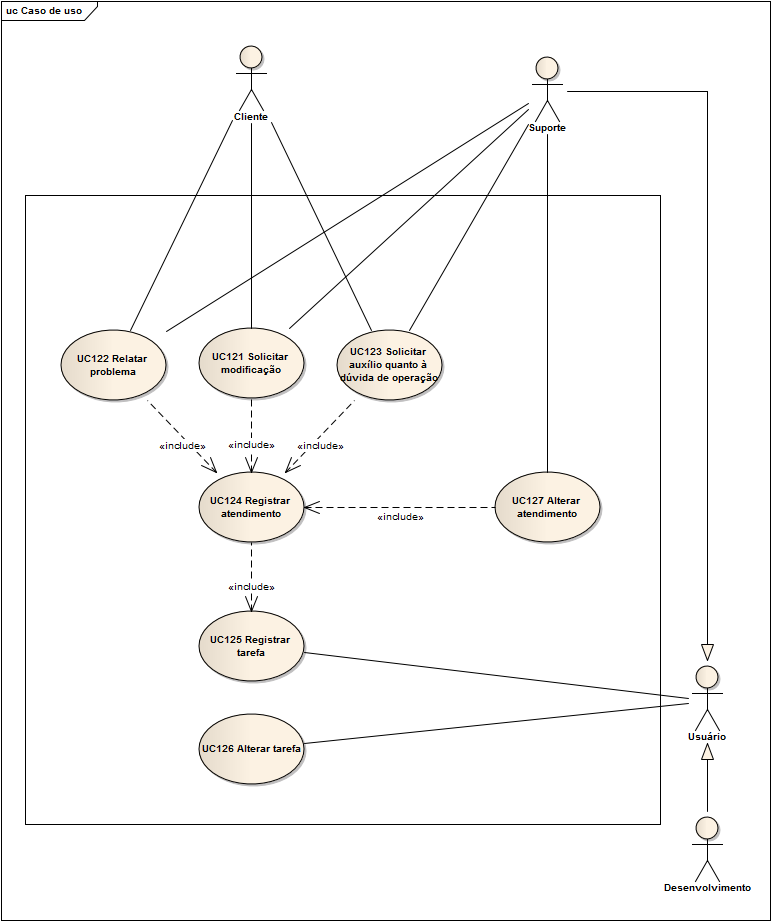
\includegraphics[scale=0.6]{figuras/UC_atendimento.png}
\caption{Caso de Uso: Atendimento}
\label{Fig:uc:atendimento}
\end{figure}

\subsection{Diagrama de Caso de Uso}

O diagrama está representado na Figura \ref{Fig:uc:atendimento}.

\subsection{Atores}

\begin{itemize}

\item[\textbf{Cliente:}] cliente interno ou externo;
\item[\textbf{Desenvolvimento:}] pessoa responsável pelo desenvolvimento de sistemas;
\item[\textbf{Suporte:}] pessoa responsável pelo atendimento do departamento de Suporte Técnico;
\item[\textbf{Usuário:}] usuário dos sistemas de atendimento, tarefas, etc.
 
\end{itemize}

\subsection{Descritivos dos Casos de Uso}

\subsubsection{UC121 Solicitar modificação}

\textbf{Principal - Solicitar modificação}

\begin{enumerate}
\item Cliente entra em contato para solicitar alguma modificação no sistema
\item Suporte registra o atendimento (UC124)
\item Suporte registra uma tarefa contendo a solicitação para o Desenvolvimento (UC125)
\end{enumerate}

\subsubsection{UC122 Relatar problema}

\textbf{Principal - Relatar problema}

\begin{enumerate}
\item Cliente entra em contato para relatar algum problema
\item Suporte registra o atendimento (UC124)
\item \{Identificado erro no sistema\} Suporte registra uma tarefa contendo o erro do sistema para o Desenvolvimento (UC125)
\end{enumerate}

\subsubsection{UC123 Solicitar auxílio quanto à dúvida de operação}

\textbf{Principal - Solicitar auxílio}

\begin{enumerate}
\item Cliente entra em contato para solicitar auxílio quanto à duvida de operação do sistema
\item Suporte registra o atendimento (UC124)
\end{enumerate}

\subsubsection{UC124 Registrar atendimento}

\textbf{Principal - Atendimento}

\begin{enumerate}
\item Suporte identifica o cliente no sistema de atendimento
\item Suporte categoriza o atendimento (dúvida, erro, solicitação, etc.)
\item Suporte redige o texto que identifica os principais pontos do atendimento que foi efetuado
\item \{Atendimento concluído sem nenhuma pendência\} Suporte fecha o atendimento
\item \{Atendimento concluído com alguma pendência\} Suporte registra as tarefas referentes às pendências identificadas durante o atendimento
\end{enumerate}

\textbf{Alternativo - Cliente bloqueado}

\begin{enumerate}
\item O cliente identificado possui algum tipo de restrição (inadimplente, bloqueado, etc.)
\item O sistema alerta:  "Cliente inadimplente/bloqueado"
\item Fim do caso de uso
\end{enumerate}

\textbf{Alternativo - Cliente não existe}

\begin{enumerate}
\item O cliente não foi identificado no sistema de atendimento
\item Sistema alerta  "Cliente não encontrado"
\item Fim do caso de uso
\end{enumerate}

\subsubsection{UC125 Registrar tarefa}

\textbf{Campos - Dados da tarefa}

\begin{itemize}
\item Responsável
\item Prioridade
\item Descrição
\item Data limite para conclusão
\item Data de previsão
\item Data de conclusão
\end{itemize}

\textbf{Principal - Registrar}

\begin{enumerate}
\item Usuário identifica responsável pela tarefa
\item Usuário preenche dados da tarefa
\item Usuário salva tarefa
\end{enumerate}

\subsubsection{UC126 Alterar tarefa}

\textbf{Principal - Alterar}

\begin{enumerate}
\item Usuário registra nova tarefa associada a uma tarefa já existente
\item Usuário fecha uma tarefa atribuída a ele
\end{enumerate}

\subsubsection{UC127 Alterar atendimento}

\textbf{Principal - Fechar}

\begin{enumerate}
\item Usuário fecha o atendimento
\end{enumerate}

\textbf{Principal - Novo registro}

\begin{enumerate}
\item Usuário inclui um novo registro a um atendimento já cadastrado (não é permitido alterar o texto do atendimento já cadastrado) (UC124)
\end{enumerate}

\textbf{Alternativo - Tarefas pendentes}

\begin{enumerate}
\item Usuário tenta fechar um atendimento que possua tarefas pendentes
\item Sistema alerta: "Não é possível fechar um atendimento com tarefas pendentes"
\end{enumerate}